\chapter{Company presentation}

\section{Presentation}

Hindsite Interactive is a small-size enterprise located in Frederick, Maryland at
approximately 45 minutes to the large city of Washington DC. Hindsite owns a
subsidiary Webnet Hosting based in Rockville, at the periphery of Washington
DC. Both Frederick and Rockville are under the area of effect of the capital
city whose total agglomeration counts more than 5 billion inhabitants.

\textbf{Headquarter} \\
Hindsite Interactive Inc.\\
241 East 4th Street\\
Frederick, Maryland 21701 USA\\

\subsection*{Short History}

Hindsite Interactive is a young company founded in 2000 by the actual
President of Operation, Mr. Payman Taei. Everything started from the corner
of a small apartment, \$170 and a vintage Pentium processor and is now a
business with two divisions. As written on Hindsite Interactive website: his main goal is not to form a conglomerate corporation but to provide a quality service and to maintain a
strong relationship with each of his client.

\section{Organizational Unit}

Hindsite is a very small company, it counts in total between 10 and 12
employees and they are not all working in the same place. The following diagram is a representation of the organization unit at Hindsite
Interactive.

\begin{figure}[ht]
\centering
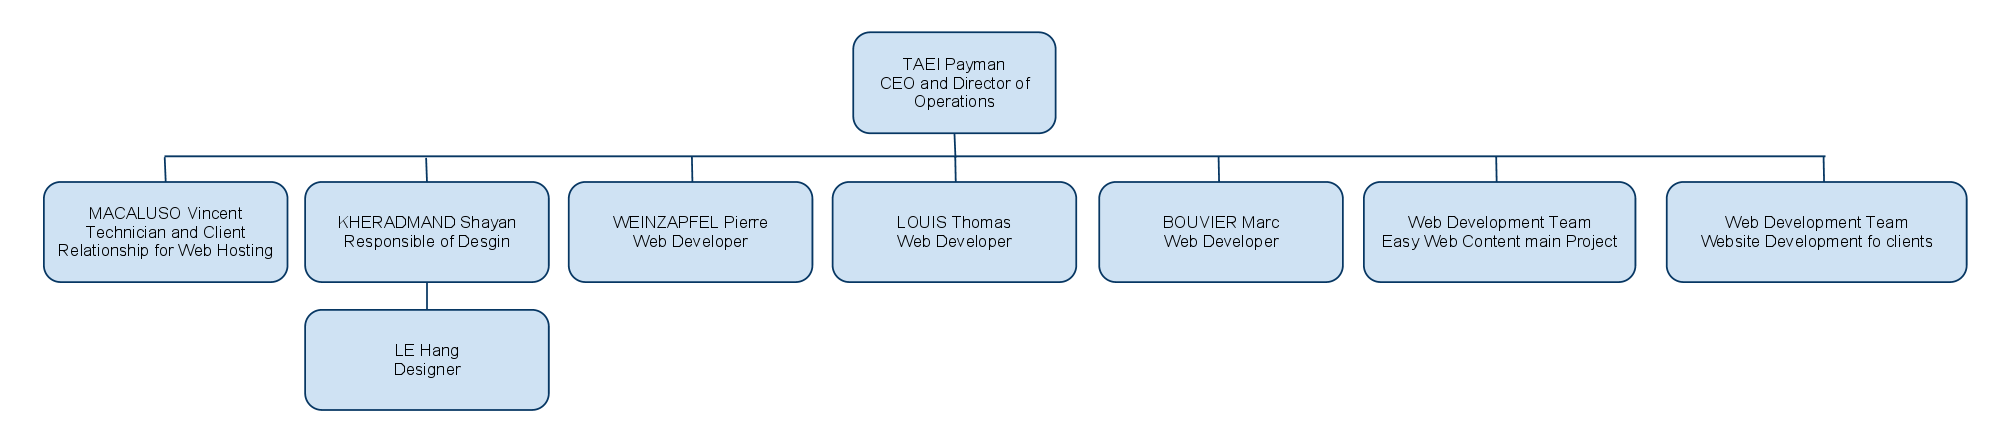
\includegraphics[width=\textwidth]{img/hindsite_organigramme.png}
\caption{Hindsite Interactive Hierarchy}
\label{figure:organigramme}
\end{figure}

My role at Hindsite Interactive takes place in the development team, as a
junior web developer. My hierarchic superior is Mr. Payman Taei, who assign
my tasks most of the time. But I am also working closely from the designer Mr.
Shayan Kheradmand to take over the design phase with the development one.
During all my internship I was working in collaboration with Mr. Pierre
Weinzapfel, web-developer and ex UTBM student.
Finally I have always been in touch with other developers at Hindsite who are
working from a different geographic place.

\section{Company activities}

Hindsite Interactive proposes different services though its different labels.
Around the Hindsite Interactive name are gathered:
\begin{itemize}
\item The web design and web development
\item Graphic design and interfaces
\item 3D modeling
\item Animation and interactivity
\end{itemize}
The website development is diversified but essentially centered on the CMS,
e-commerce and dynamic applications.

\subsection*{Webnet Hosting}

This subsidiary from Hindsite Interactive takes care of the management and
hosting of websites. In addition, the company offers a large number of
services that are a success with not less than a thousand websites hosted.

Overview of the main services and characteristics:
\begin{itemize}
\item Easy Web Content: the website editor
\item A CMS: Site Studio Design that proposes 600 templates
\item Urchin for analysis and statistics
\item Word Press for the realization of forums, blogs, pools etc.
\item CPanel, for site configuration and management
\item Full backup every night
\end{itemize}
Since his creation Hindsite proposes solutions in term of design and animation
that use the newest technologies and therefore has a recognized know-how in
his field of competence.
A proof is Hinsite’s website entirely realized in Flash and animated. This site is
a portfolio itself of the company competences.
The company received awards for his website and the quality of work from
“PC World”, “Best of the Web”, “Perfectory Award” and the “Golden Web
Award” by The International Association of Web Masters and Designers.

\section{Clients}

Even Hindsite is still a young company, it owns already an extended contact
list. Here are some example of customer and projects:

%abc news image
\paragraph*{ABC News}
A division of the famous television channel ABC, one of the
four top networks in the US. ABC News is a national news channel. Hindsite
realized a module for the website to cover the last presidential campaign.
\paragraph*{Avalere}
A leading advisory company focused on healthcare business
strategy and public policy. Our company realizes different projects for
Avalere’s customers.
\paragraph*{Noland Aviation} an aircraft sales and acquisition company. Hindsite
Interactive entirely designed and developed the website and Flash animations.
\paragraph*{Sentara College of Health Sciences} a university located in Virginia. It
belongs to the Sentara Health System organization that counts a hundred of
sites. Hindsite designed a website with a full CMS.
\paragraph*{Bay Area Biomedical Consultants Network} provides
networking and educational opportunities for consultants in the San Francisco
life sciences community. Another example of a website developed by Hindsite
Interactive and in which I participated in the development.

Through these examples we see that clients come from various fields like
industry, services, consulting, education, health, Medias, etc.
This shows that Hindsite knows how to adapt to the specific needs of the
different clients.

\section{Services proposed}

\subsection{Complete website development}

Hindsite proposes its clients to create their websites from A to Z, including the
specification, the design, the development, eventually an administration
section and hosting on its server.

\subsection{Other design projects}

This can be a CD/DVD presentation, a logo, a Flash animation or banner, a
company presentation in a video format, advertisements, etc.

\subsection{Easy Web Content}
%easy web content image
\begin{figure}[!ht]
\centering

\includegraphics[width=.30\textwidth]{img/ewc.png}
\caption{Easy Web Content Logo}
\label{figure:ewc-logo}
\end{figure}

Easy Web Content is a solution that can be compared to a CMS (Content
Management System). This innovative web platform allows website owners to
update easily and maintain their websites.

The solution proposed is entirely online and doesn’t require any download and
installation. As a matter of fact, the system is modular and flexible.
It is important to highlight that the system does not require any knowledge in web
development and everything is done to facilitate usability. Most of the users are
novice.

Easy Web Content allows users to manage their web pages, edit content, manager
their FTP server but also to add dynamic content to their pages as a music player, a calendar etc. Major possibilities of the software.

\begin{itemize}
\item Edition of all pages and content
\item Creation of web pages
\item Addition of interactive, dynamic content in Flash and/or HTML (all add-ons)
\item Security of pages with a login/password access
\end{itemize}

\section{Company Analyze}

Hindsite Interactive has a strategic geographic position, indeed Frederick is
located inside an agglomeration with a worldwide influence in the eastern
megalopolis of the USA and its main city New York City. This area is the
economical heart of the country and counts more than 55 million inhabitants.

It’s also one of the most influent in the world in the economical, financial,
political or even cultural aspects. All this favorites businesses of all kind and
especially requires new technologies and information systems (IT). As a
matter of fact, Hindsite Interactive occupies a central position that allows it to
answer quickly and efficiently to the customer needs.

Closer to Frederick, Washington DC is the capital of the USA and therefore
hosts thousands of federal institutions, organizations, law firms, medias,
consulting companies etc. Moreover the Washington area comprises
worldwide companies headquarters and some of the most famous universities
(e.g. Georgetown).

Hindsite knew how to take advantage of this heterogeneity by offering different
services and have client in all sectors. This non-specialization offers Hindsite
the ability to continue growing during the economical crisis.
In order to comply with the Business Model of the company, the philosophy is
to develop the interdisciplinary of competences and a quick adaptation to the
new technologies to answer the best to the client expectations.

\clearpage